\documentclass[10pt,a4paper]{article}
\usepackage[margin=16mm]{geometry}\usepackage{fontspec,amsmath,graphicx,booktabs,longtable,hyperref}
\setmainfont{Latin Modern Roman}\setlength{\parindent}{0pt}\setlength{\parskip}{5pt}
\begin{document}
{\LARGE Local cone-referenced angular residuals}\par
7 October 2026. Diagnostic trial; all intensity fits and background parameters are unchanged.

This supplement tests the requested alternative to exact inversion. At each matched fitted cone direction $d_j$, take the corrected held-out anisotropy minus the fitted signal anisotropy:
\[e_j=XY(I^{heldout}_j-B-L_j^{fit})-XY(S_j^{fit}).\]
The interference term is still evaluated at the fitted direction. This is a conditional diagnostic, not a self-consistent refit of interference.

Let $k$ be the fitted cone axis, $\lambda$ its half-angle, and define unit tangent directions
\[t_\perp=(\cos\lambda\,d-k)/\sin\lambda,\qquad t_\parallel=(k\times d)/\sin\lambda.\]
The first points towards increasing cone angle; the second follows increasing mechanical phase. Using the signal-only anisotropy map $F(d)$, calculate its local two-by-two Jacobian and solve
\[J_j=\left[\partial_{t_\perp}F\quad\partial_{t_\parallel}F\right],\qquad
\begin{pmatrix}\delta\lambda\\\delta s\end{pmatrix}=J_j^{-1}e_j,
\qquad \delta s\simeq\sin\lambda\,\delta\psi.\]
This uses anisotropy residuals, not a new four-channel intensity objective. It does not constrain total brightness or pair balance. Brightness factors cancel in signal anisotropy. The analytic annular Fourkas map is used consistently for the derivative; residuals are measured relative to the actual numerical fitted signal so quadrature differences do not create a spurious zero-residual shift.

To display the displacement on the unit sphere, use its tangent-plane exponential map:
\[v=\delta\lambda\,t_\perp+\delta s\,t_\parallel,\quad a=\|v\|,\qquad
 d_{local}=\cos a\,d+\frac{\sin a}{a}v.\]
This stays on the sphere but need not stay on the cone. No clipping, smoothing or residual shrinkage is applied. This is a first-order angular estimate, not an exact inverse. It can form a closed path because the reference geometry and residual are periodic; closure here is not independent evidence that the model is correct.

\textbf{Check the approximation.} Re-evaluate the nonlinear signal map and calculate
\[\eta_j=\frac{\|F(d_{local})-F(d_j)-e_j\|}{\max(\|e_j\|,10^{-8})}.\]
A small $\eta$ means the displayed local displacement reproduces the requested anisotropy change. Red points flag any of: angular step above $15^\circ$, $\eta>25\%$, Jacobian condition number above100, rank deficiency, or invalid corrected channels/radius. These are explicit exploratory caution thresholds, not confidence intervals. Exponential mapping of large steps can wrap around the sphere and is not physically trustworthy. The lower panel exposes this instead of hiding it.

\textbf{Comparison.} Grey points show the previous continuous exact inverse, where valid; blue/red points show the local approximation. Red points may be drawn even when exact inversion is invalid: these are extrapolations, not newly valid measurements. The middle panels show local tangent components, not the earlier circle-centre elevation $\beta$.

All90 window/cap cases were evaluated numerically. Figures show the10\% case for each family where applicable, plus uncapped no-BG and Richard. The full original cap-sweep report is unchanged.
\newpage
\section*{Representative results}
\begin{longtable}{llrrrr}\toprule
Model & Window & RMS (deg) & Max (deg) & Flagged & Median $\eta$\\\midrule\endhead
No background & 30s & 20.6 & 37.0 & 62/128 & 0.22\\
No background & 10s & 20.4 & 34.4 & 63/128 & 0.22\\
Additive background & 30s & 10.6 & 19.8 & 20/128 & 0.14\\
Additive background & 10s & 13.0 & 20.3 & 41/128 & 0.15\\
Richard four-C & 30s & 129.4 & 426.0 & 107/128 & 0.65\\
Richard four-C & 10s & 76.4 & 212.3 & 111/128 & 0.62\\
Additive + bounded interference & 30s & 573.0 & 4784.8 & 93/128 & 0.56\\
Additive + bounded interference & 10s & 46.4 & 127.8 & 96/128 & 0.54\\
Uniform field & 30s & 1640.5 & 18376.3 & 79/128 & 0.83\\
Uniform field & 10s & 356.0 & 3886.7 & 84/128 & 0.37\\
Three-mode field & 30s & 235.4 & 2271.7 & 78/128 & 0.39\\
Three-mode field & 10s & 125.3 & 991.5 & 71/128 & 0.26\\
Five-mode field & 30s & 10.0 & 27.0 & 25/128 & 0.03\\
Five-mode field & 10s & 10.2 & 21.9 & 30/128 & 0.06\\
General stationary field & 30s & 2.9 & 7.3 & 0/128 & 0.02\\
General stationary field & 10s & 3.5 & 8.3 & 0/128 & 0.03\\
Hole-edge field & 30s & 11.5 & 22.1 & 33/128 & 0.09\\
Hole-edge field & 10s & 12.7 & 22.8 & 43/128 & 0.09\\
General field + axial motion & 30s & 1.7 & 5.4 & 0/128 & 0.01\\
General field + axial motion & 10s & 2.8 & 5.9 & 0/128 & 0.03\\
\bottomrule\end{longtable} The angular RMS includes flagged finite estimates; it is not an accuracy ranking. Singular directions have no usable local inverse. See each figure for where the linear approximation fails.
\newpage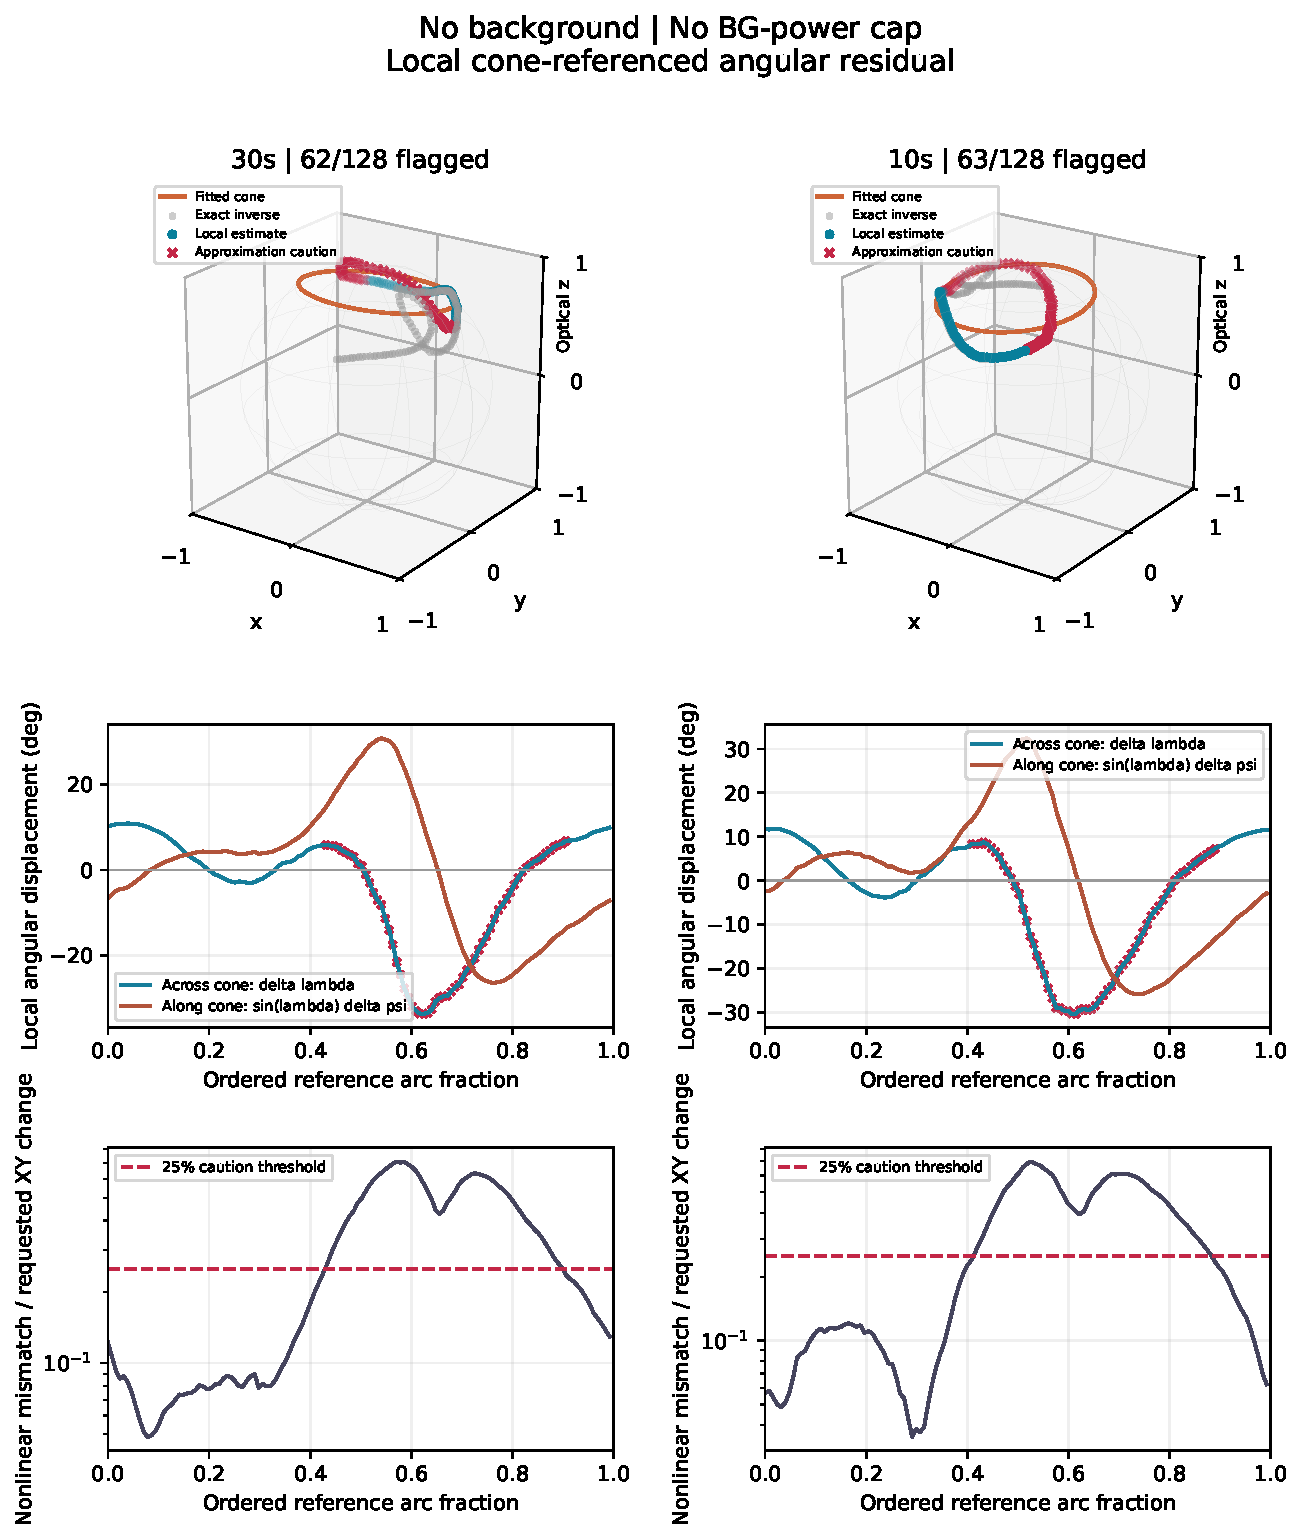
\includegraphics[width=\linewidth,height=.96\textheight,keepaspectratio]{none.pdf}
\newpage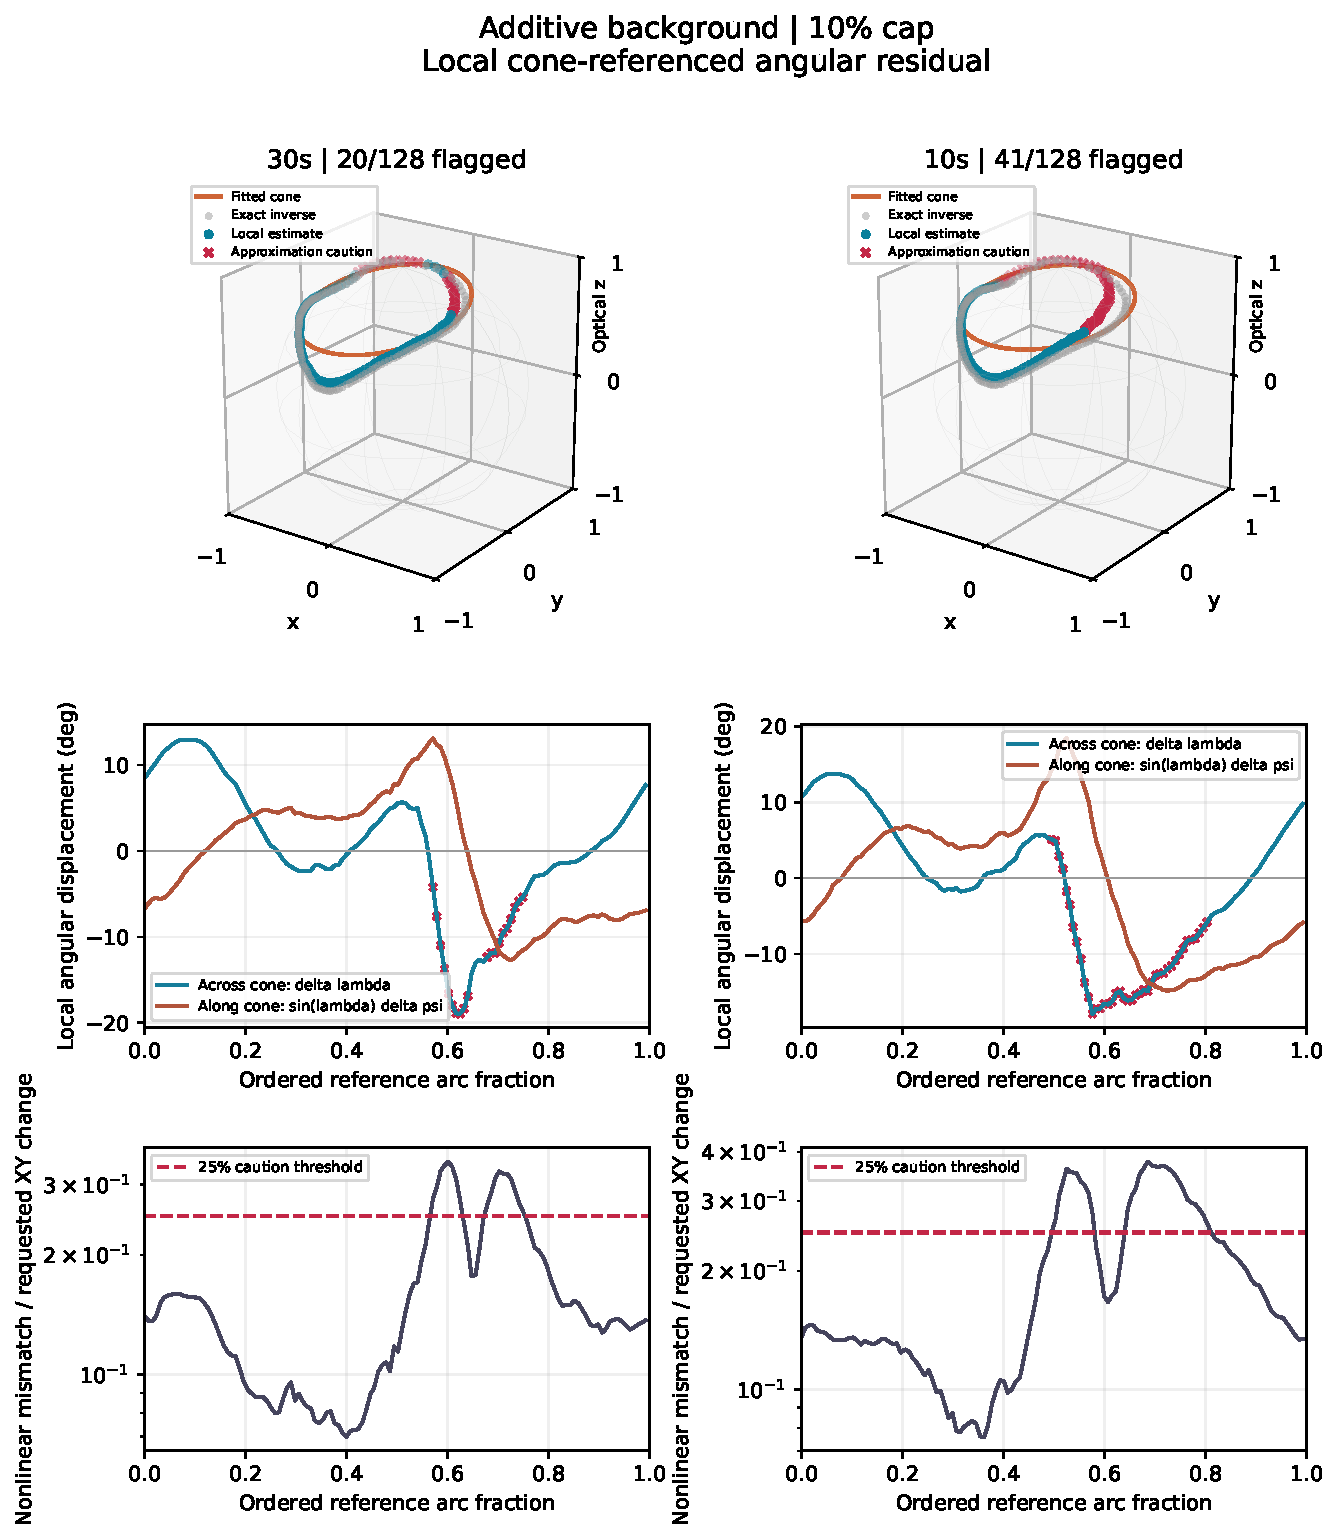
\includegraphics[width=\linewidth,height=.96\textheight,keepaspectratio]{square.pdf}
\newpage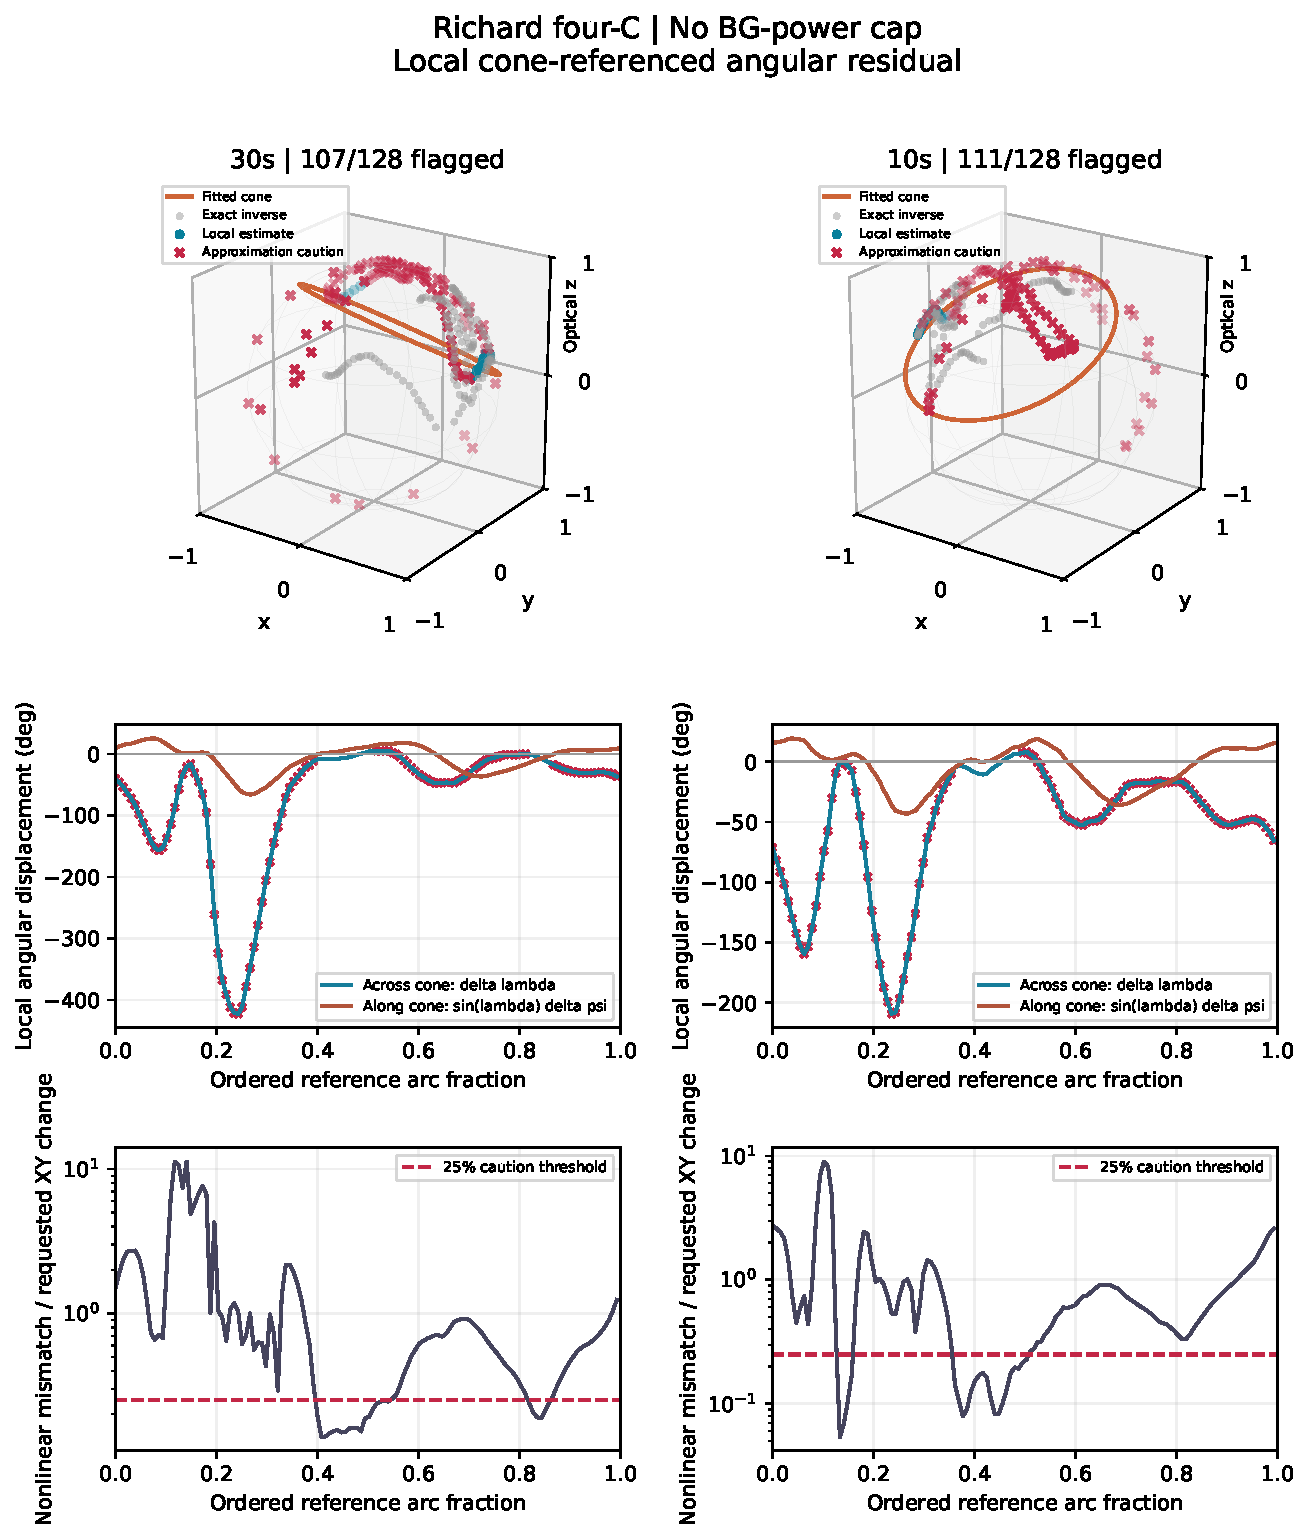
\includegraphics[width=\linewidth,height=.96\textheight,keepaspectratio]{richard_product.pdf}
\newpage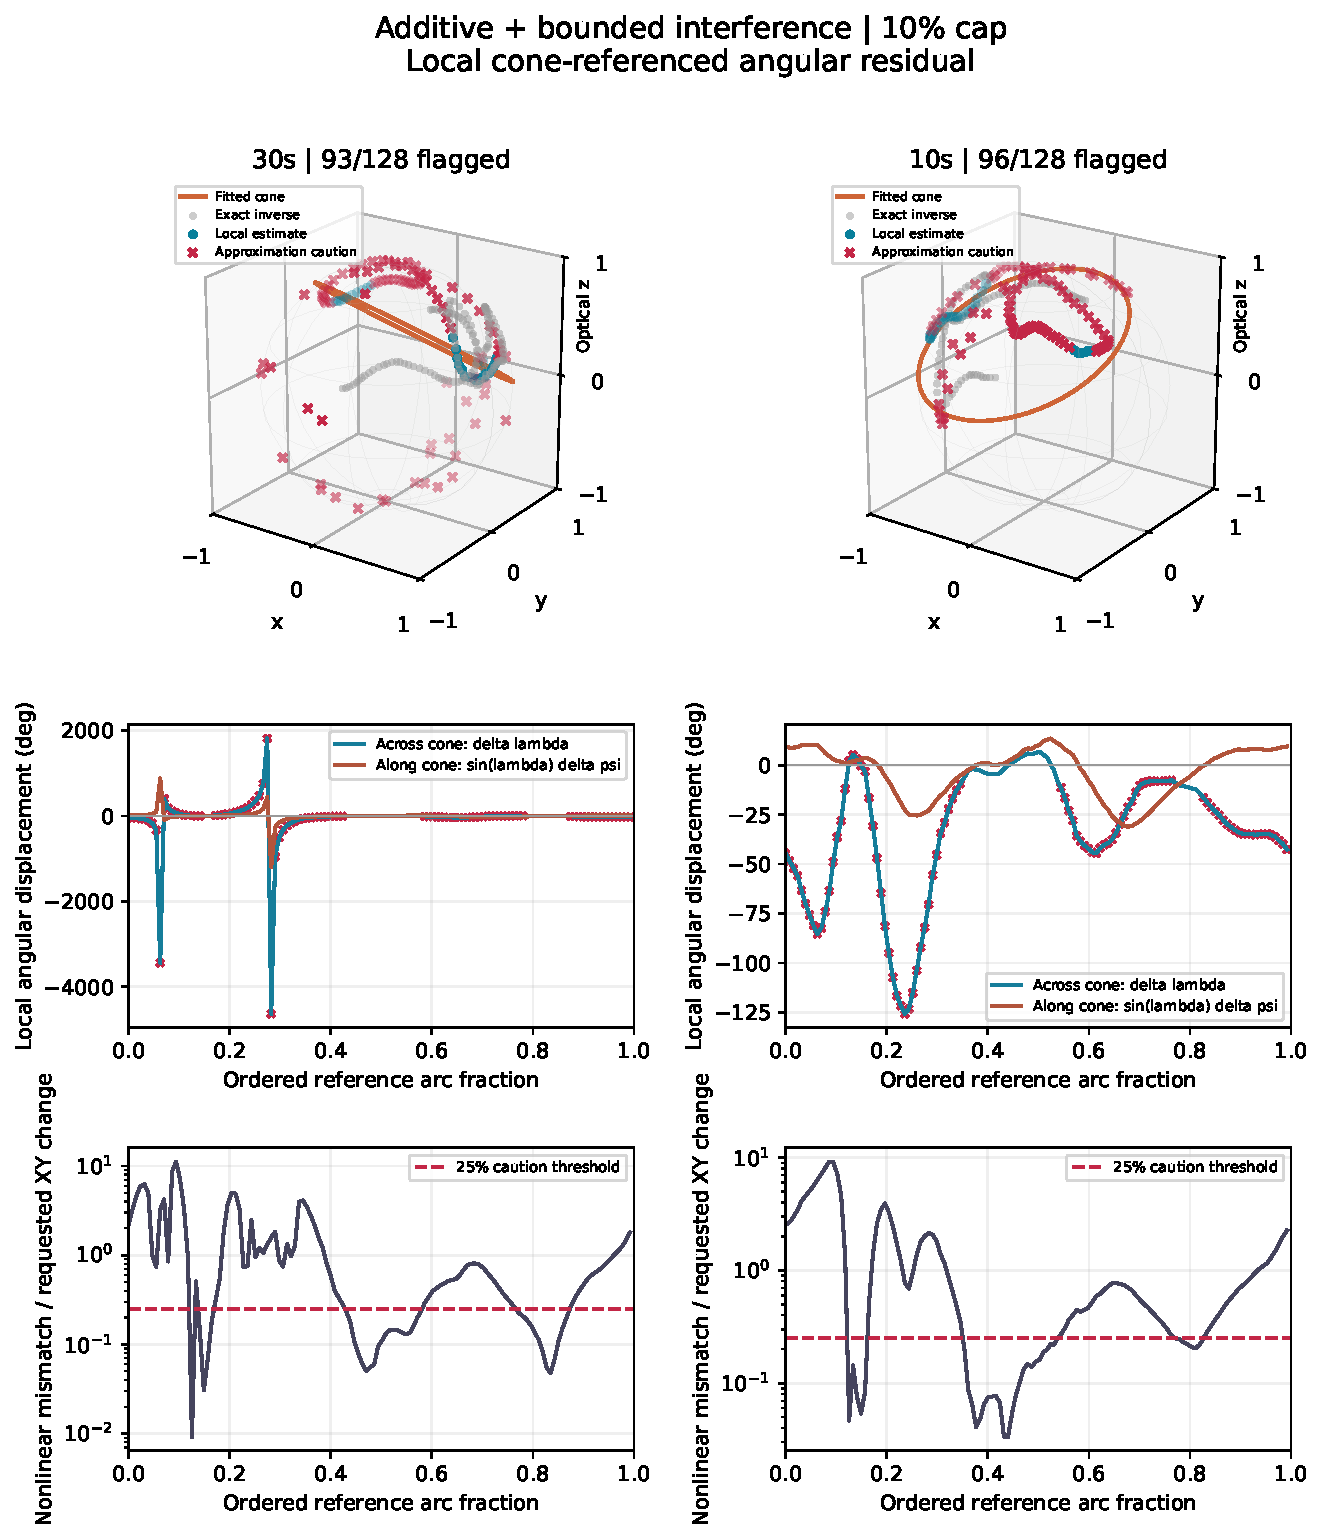
\includegraphics[width=\linewidth,height=.96\textheight,keepaspectratio]{complex.pdf}
\newpage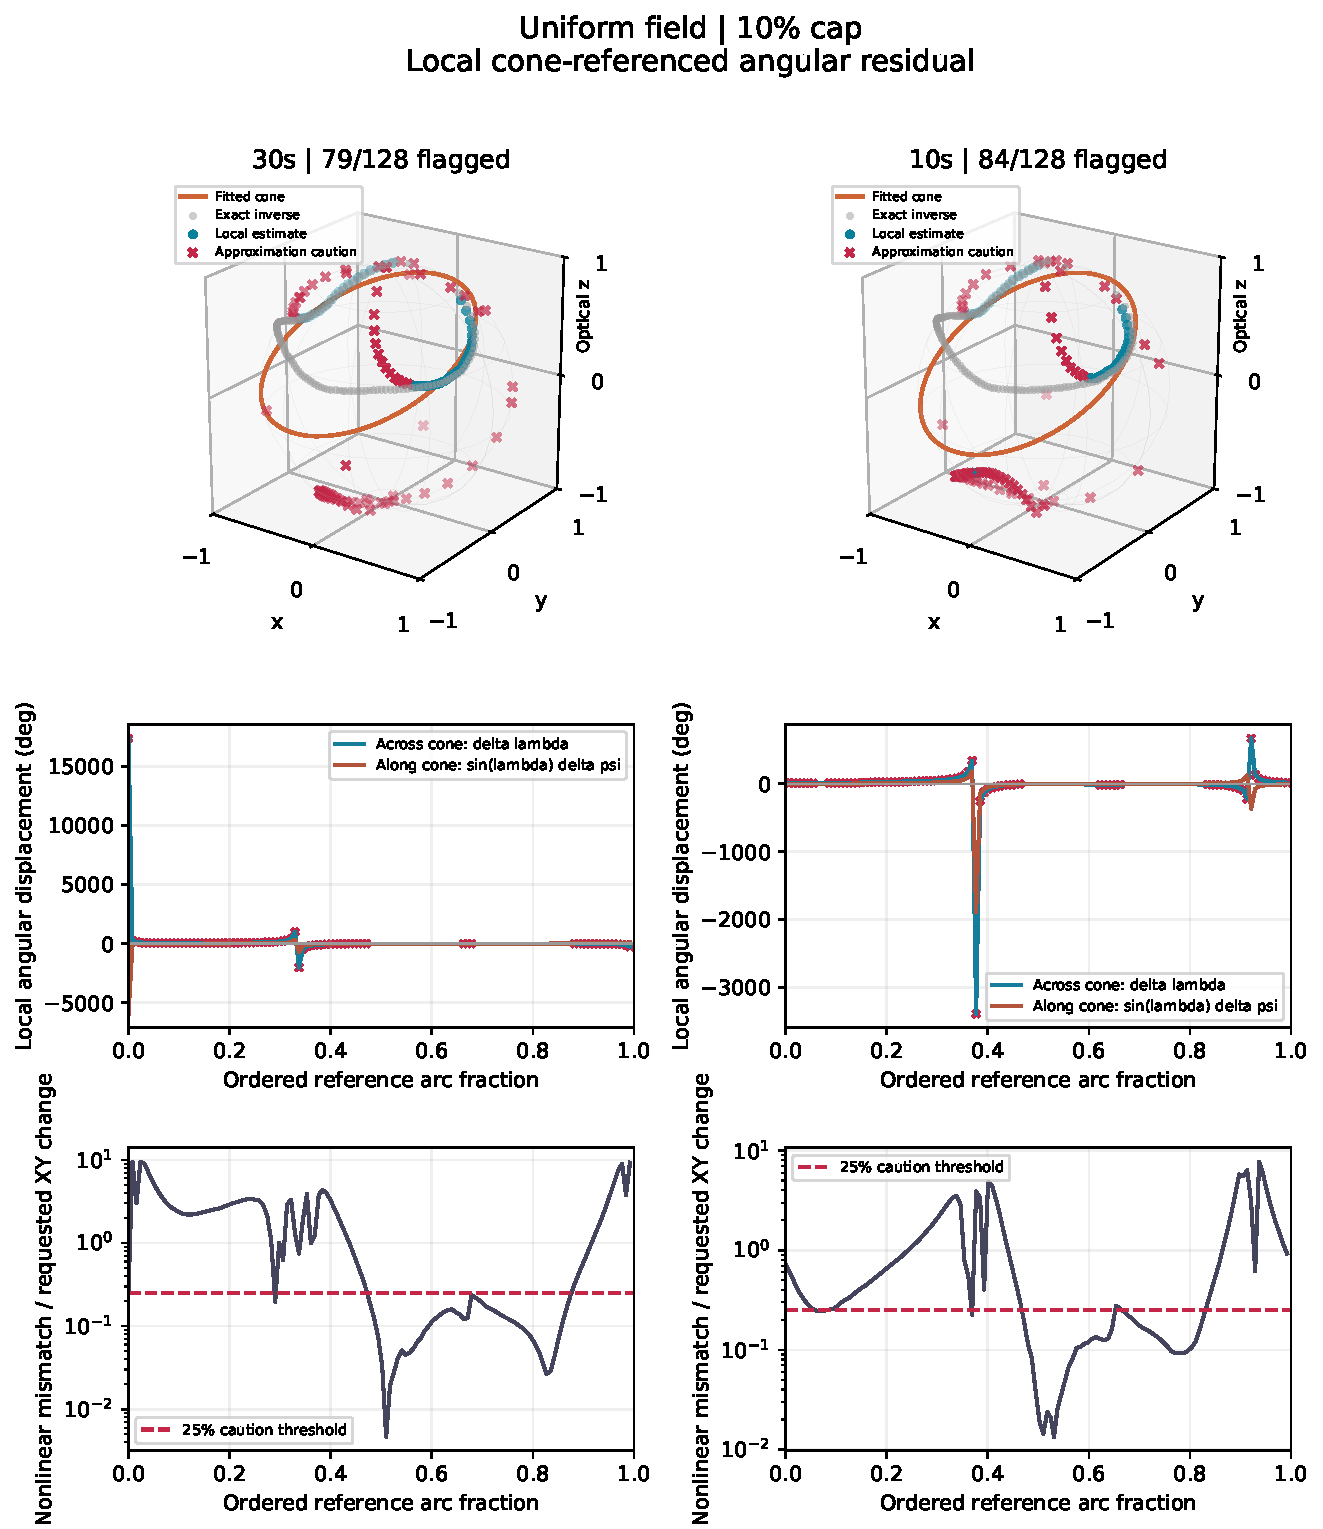
\includegraphics[width=\linewidth,height=.96\textheight,keepaspectratio]{uniform.pdf}
\newpage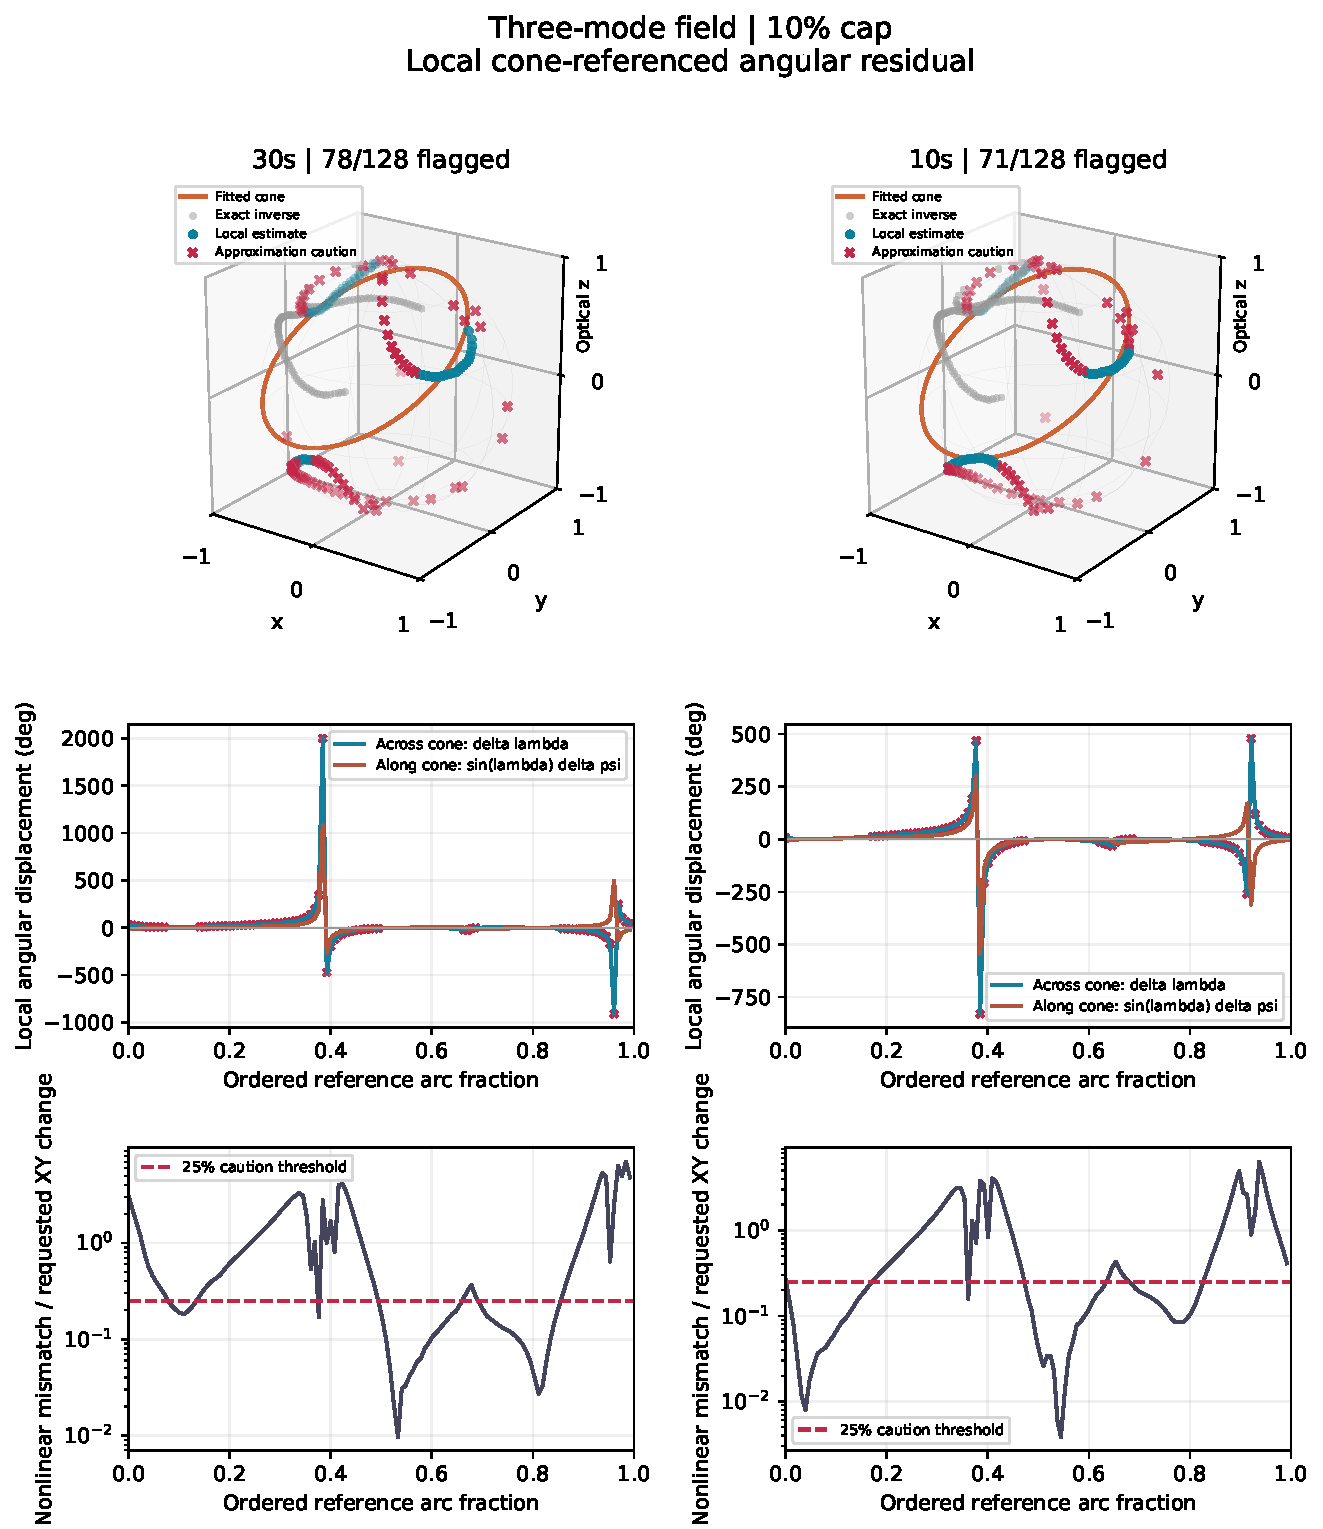
\includegraphics[width=\linewidth,height=.96\textheight,keepaspectratio]{three.pdf}
\newpage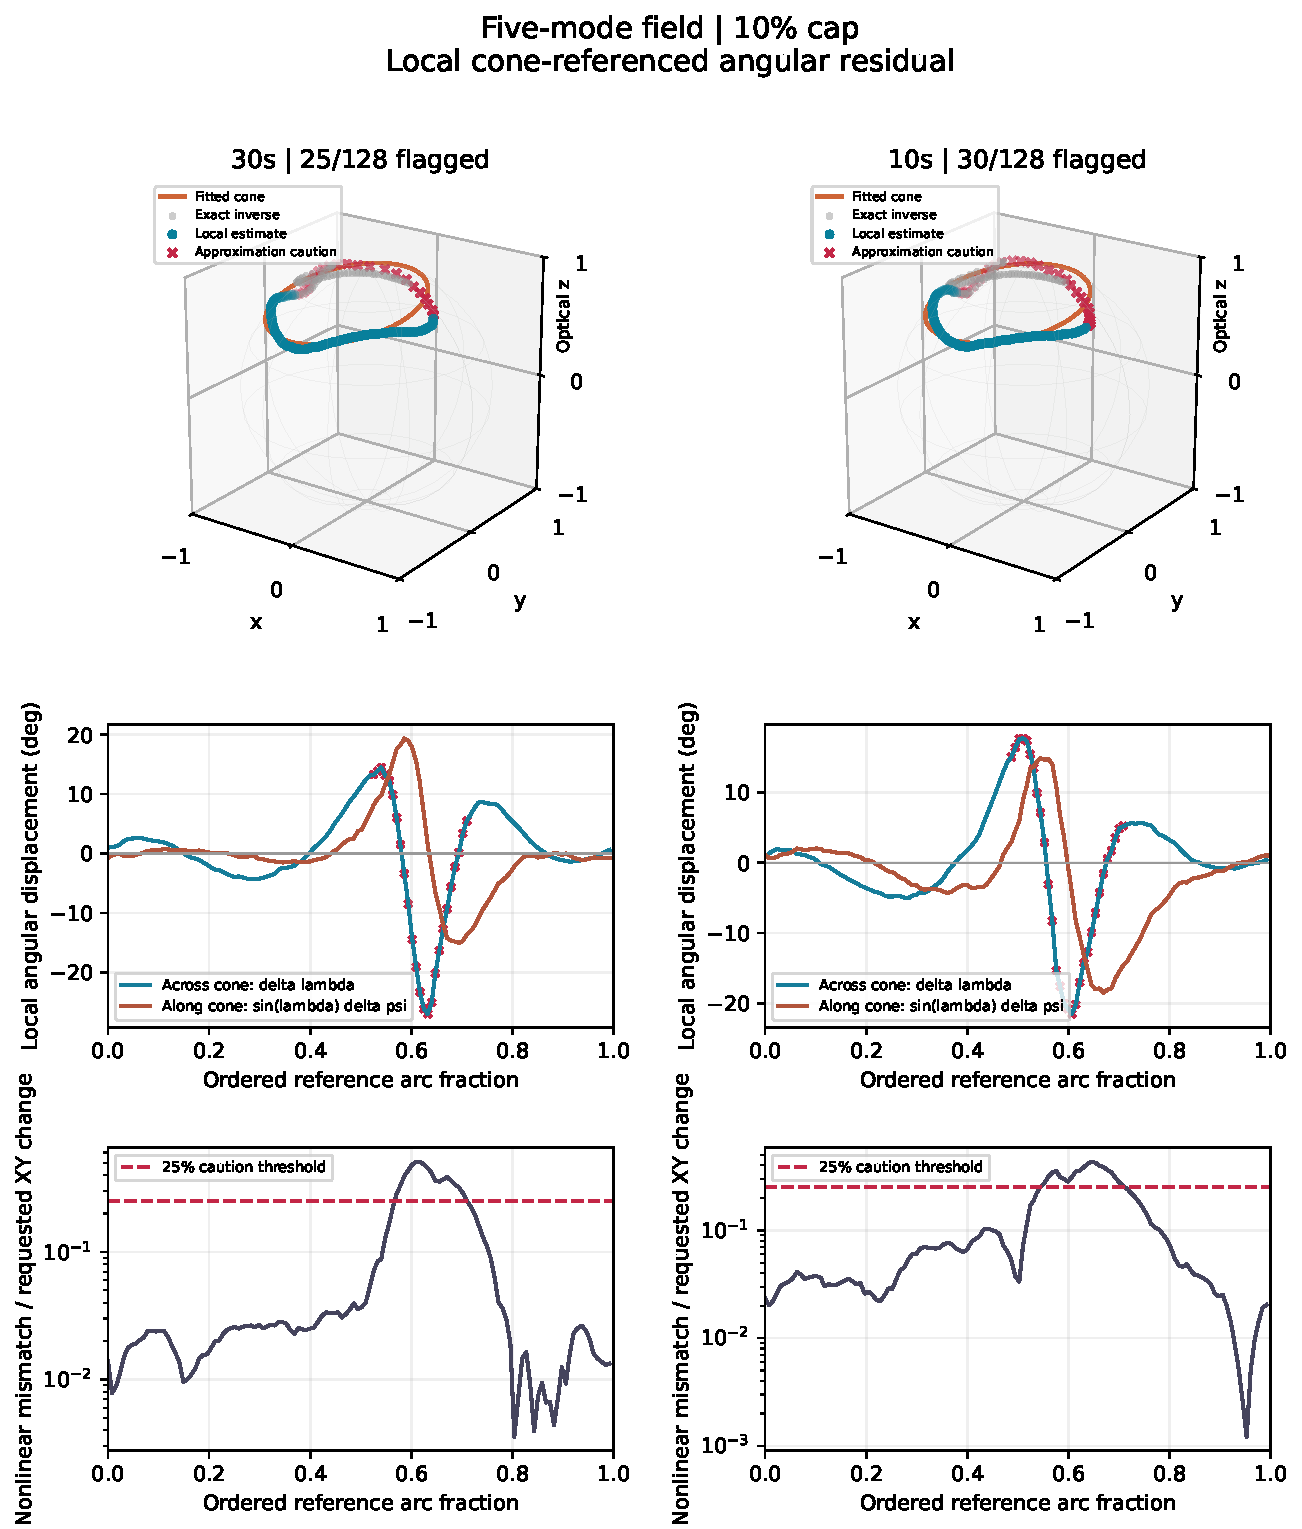
\includegraphics[width=\linewidth,height=.96\textheight,keepaspectratio]{five.pdf}
\newpage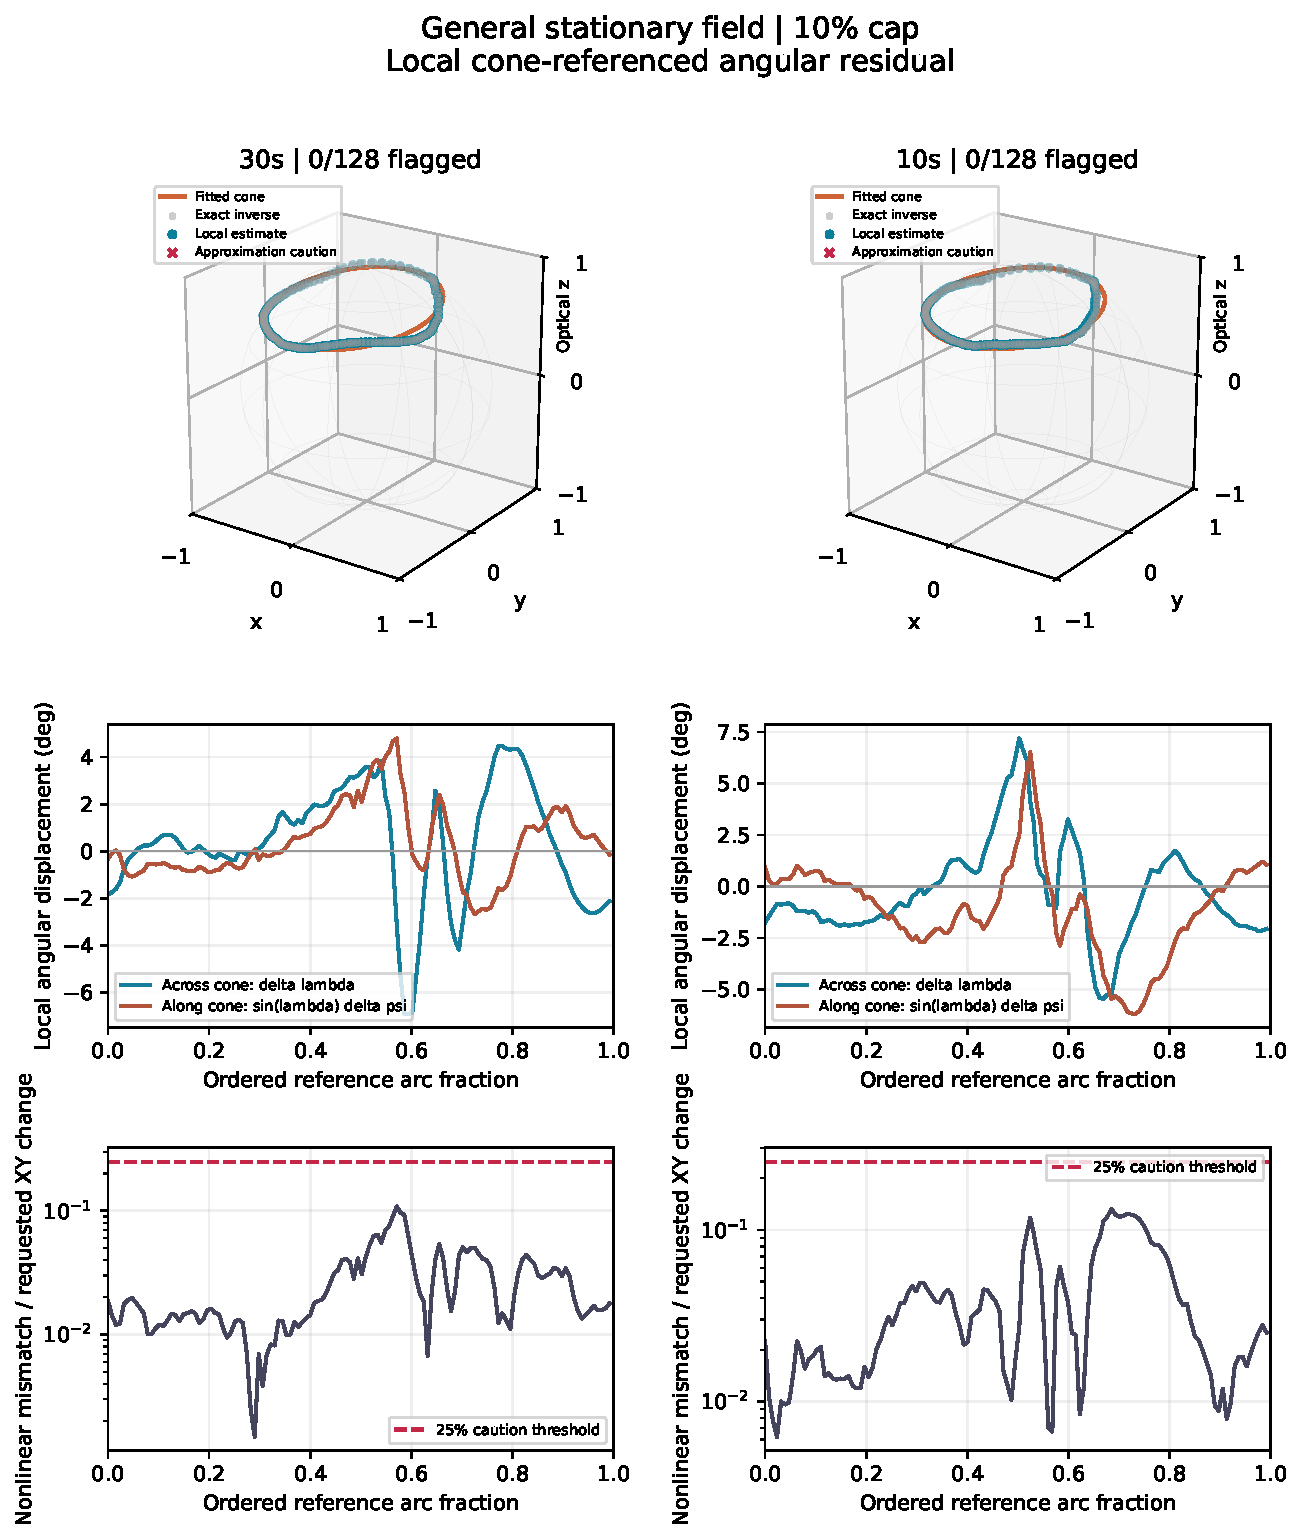
\includegraphics[width=\linewidth,height=.96\textheight,keepaspectratio]{general.pdf}
\newpage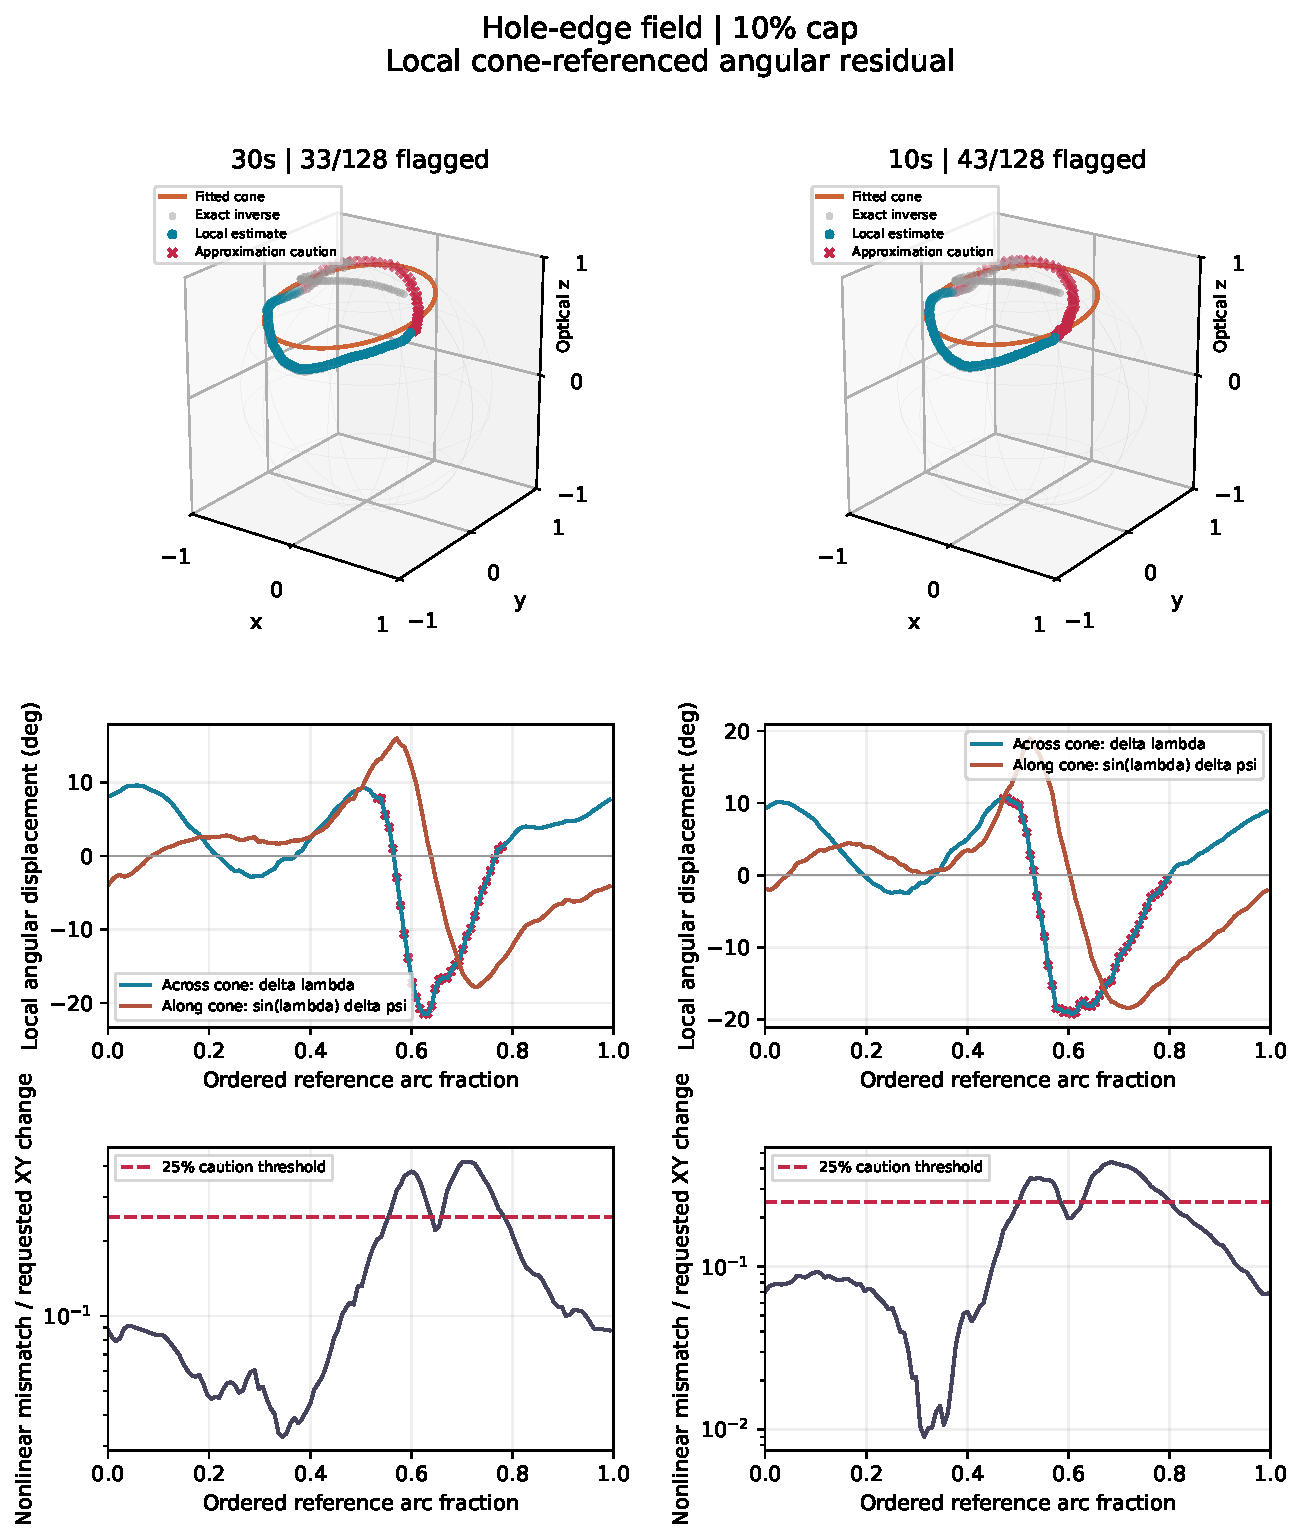
\includegraphics[width=\linewidth,height=.96\textheight,keepaspectratio]{edge.pdf}
\newpage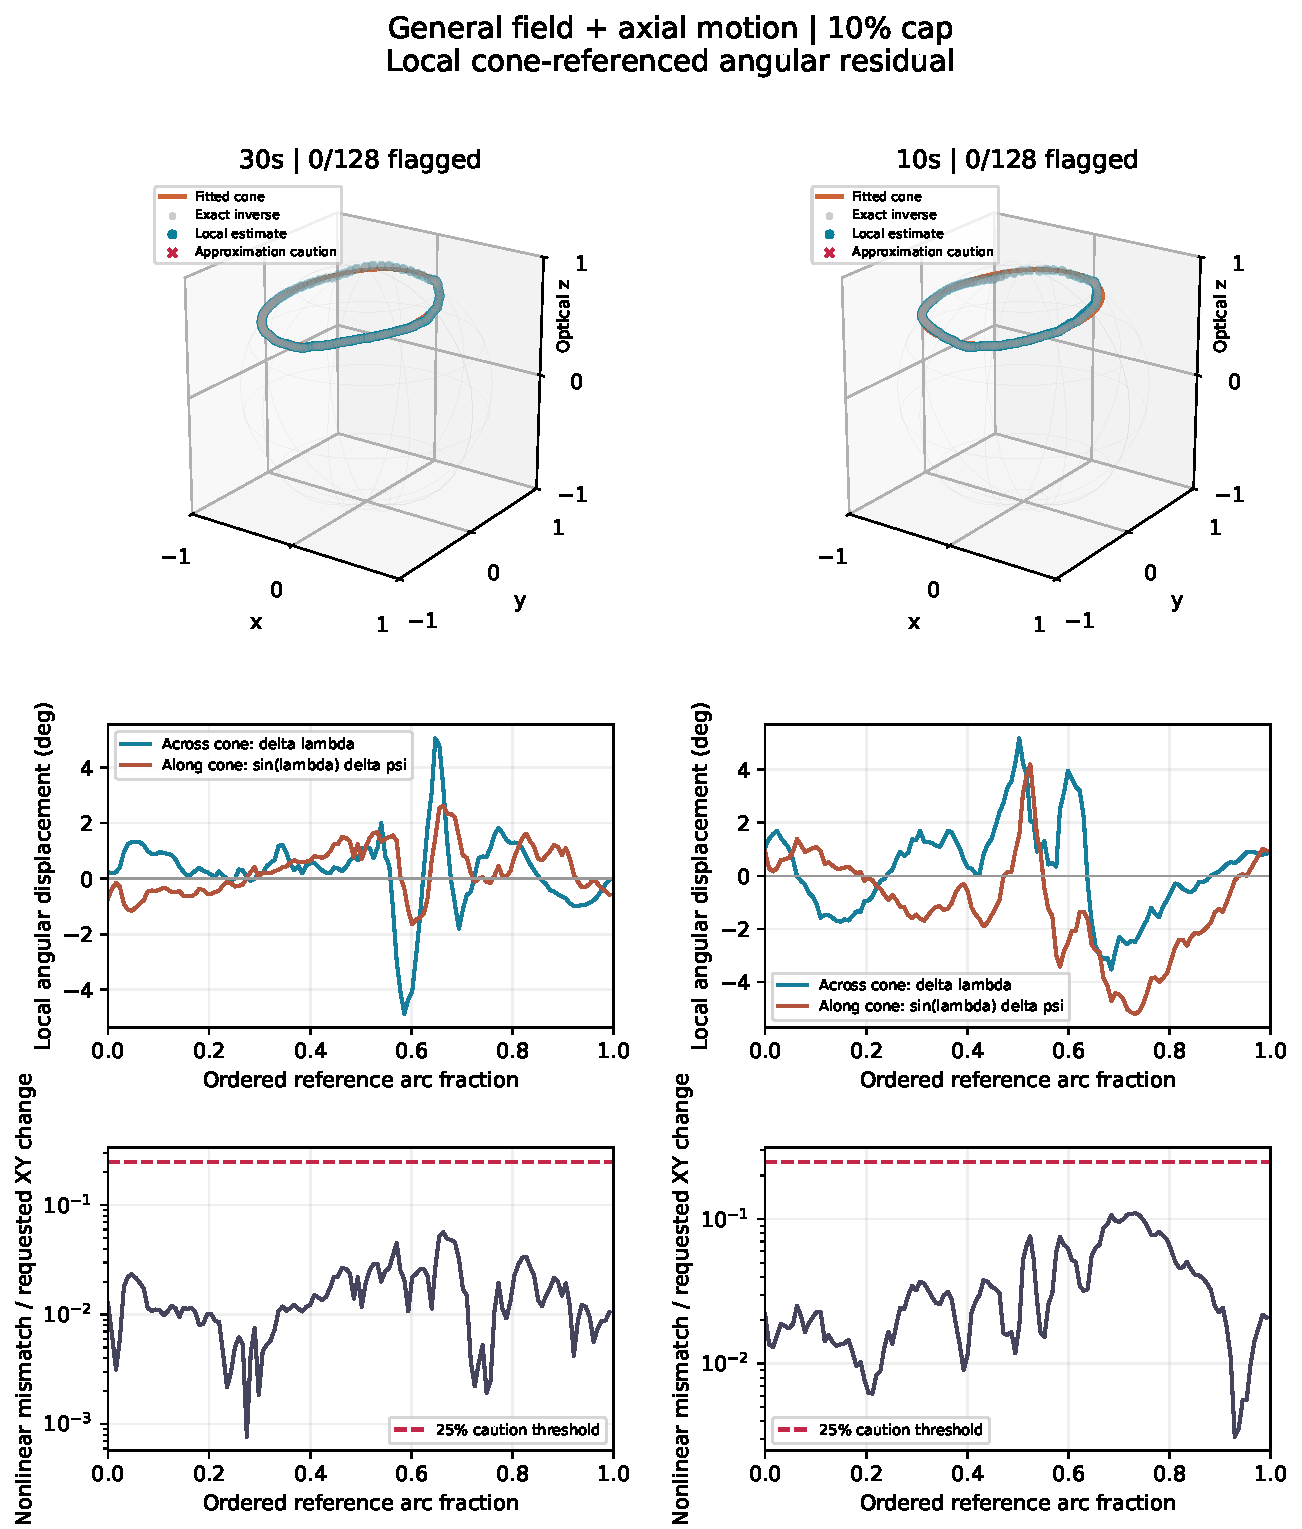
\includegraphics[width=\linewidth,height=.96\textheight,keepaspectratio]{axial.pdf}
\end{document}
